\documentclass[a4paper]{ctexart}
%\usepackage{fdsymbol}
\usepackage{graphicx}
\usepackage{epstopdf}
\usepackage{mathtools,amsmath,amsthm,amsfonts,bm}
\usepackage{booktabs}
\usepackage{xcolor}
\usepackage{multirow}
\usepackage{threeparttable}
\usepackage{listings}
\usepackage{cases}
\usepackage[left=1in,right=1.25in,top=0.25in,bottom=1in]{geometry}%设置页边距
\title{\textbf{Advanced Econometrics}}
\author{\textbf{Problem Set 1}\\(Due Monday, October 21 in class)}
\date{}

\theoremstyle{remark}
\newtheorem*{solution}{解}
\renewcommand{\qedsymbol}{证毕}

\pagenumbering{arabic}
\pagestyle{plain}

\begin{document}
\maketitle



\begin{itemize}
%% 第一题
\item[\textbf{1.}] In the potential outcomes framework, suppose that program eligibility is randomly assigned but participation cannot be enforced. To formally describe this situation, for each person $i$, $z_i$ is the eligibility indicator and $x_i$ is the participation indicator. Randomized eligibility means $z_i$ is independent of $(Y_{0i}, Y_{1i})$ but $x_i$ might not satisfy the independence assumption.
\begin{enumerate}
\item[i.] Explain why the difference in means estimator is generally no longer unbiased.
\item[ii.] In the context of a job training program, what kind of individual behavior(s) would cause bias?
\end{enumerate}

%%第一题解答
\begin{solution}
    i. 项目资格的随机发放实际上不构成RCT,个体的参与行为实际影响Y的变化\\
    令
    \begin{equation*} 
        x_i = 
        \begin{cases}
            1, &\text{参与了活动.} \\
            0, &\text{未参与活动.}
        \end{cases}
    \end{equation*}
    \begin{equation*}
        Y_i = 
        \begin{cases}
            Y_{1i}, &{x_i = 1} \\
            Y_{0i}, &{x_i = 0}
        \end{cases} 
    \end{equation*}
    其条件期望为:
    \begin{align*}
        E(Y_i|x_i=1) - E(Y_i|x_i=0) = E(Y_{1i}|x_i=1)-E(Y_{0i}|x_i=0)\\
        =E(Y_{1i}-Y_{0i}|x_i=1)+E(Y_{0i}|x_i=1)-E(Y_{0i}|x_i=0)
    \end{align*}
    已知此时$E(Y_{0i}|x_i=1)-E(Y_{0i}|x_i=0)$为选择性偏误,代表参加项目和未参加项目人员本身的差距。由题目知$x_i$可能不满足独立性假设。\\
    因此,$E(Y_{0i}|x_i=1)\neq E(Y_{0i}|x_i=0)$。\\
    此时$E(Y_i|x_i=1) - E(Y_i|x_i=0) \neq E(Y_{1i}-Y_{0i}|x_i=1)$。即均值估计量差异有偏。\\
    \\
    ii. 由上文知选择性偏差的实际意义是个人特质由于选择造成的偏差。假设Y是个人的职业能力,由于在培训项目中参与无法被强制,那么具有较强职业能力的人员若偏向不参与,而初始能力较差的人员偏向于参与,那么就会导致$E(Y_{0i}|x_i=1)-E(Y_{0i}|x_i=0)$值为负。
    从而缩小了$E(Y_i|x_i=1) - E(Y_i|x_i=0)$的大小,使得估计量实际偏小。
    \\
    \qedsymbol
\end{solution}

%%第二题
\item[\textbf{2.}] The potential outcomes framework can be extended to more than two potential outcomes. In fact, we can think of the policy variable, $w$, as taking on many different values, and then $y(w)$ denotes the outcome for policy level $w$. For concreteness, suppose $w$ is the dollar amount of a grant that can be used for purchasing books and electronics in college, $y(w)$ is a measure of college performance, such as grade point average. For example, $y(0)$ is the resulting GPA if the student receives no grant and $y(500)$ is the resulting GPA if the grant amount is \$500.

~~~~For a random draw $i$, we observe the grant level, $w_i\geq 0$ and $y_i=y(w_i)$. As in the binary program evaluation case, we observe the policy level, $w_i$, and then only the outcome associated with that level.

\begin{enumerate}
\item[i.] Suppose a linear relationship is assumed:
\[y(w)=\alpha+\beta w+\nu(0),\]
where $y(0)=\alpha+\nu$. Further, assume that for all $i$, $w_i$ is independent of $\nu_i$. Show that for each $i$, we can write
\begin{align*}
y_i&=\alpha_i+\beta w_i+\nu_i,\\
E(\nu_i|w_i)&=0.
\end{align*}
\item[ii.] In the context of i, how would you estimate $\beta$ (and $\alpha$) given a random sample? Justify your answer. 
\item[iii.] Now suppose $w_i$ is possibly correlated with $\nu_i$, but for a set of observed variables $x_{ij}$,
\[E(\nu_i|w_i, x_{i1},...,x_{ik})=E(\nu_i|x_{i1},...,x_{ik})=\eta+\gamma_1 x_{i1}+...+\gamma_k x_{ik}.\]
The first equality holds if $w_i$ is independent of $\nu_i$ conditional on $(x_{i1},...,x_{ik})$ and the second equality assumes a linear relationship. Show that we can write
\begin{align*}
y_i&=\phi+\beta w_i+\gamma_1 x_{i1}+...+\gamma_k x_{ik}+u_i,\\
E(u_i|w_i, x_{i1},...,x_{ik})&=0.
\end{align*}
What is the intercept $\phi$?
\item[iv.]  How would you estimate $\beta$ (along with $\phi$ and the $\gamma_j$'s in part iii? Explain.
\end{enumerate}

%%第二题解答
\begin{solution}
    i. 由题设知,解释变量和被解释变量之间满足线性关系,有ols估计知,有$SSR(\alpha_i,\beta_i)$最小化。即
    \begin{equation*}
        SSR(\alpha_i,\beta_i) = \sum_{i=1}^{N} (y_i - \alpha_i - \beta_i w_i)^2
    \end{equation*}
    对SSR取最小值,有一阶条件:
    \begin{equation*}
        \frac{\partial SSR(\hat\alpha_i,\hat\beta_i)}{\partial \alpha_i} = 0,\\
        \frac{\partial SSR(\hat\alpha_i,\hat\beta_i)}{\partial \beta_i} = 0.
    \end{equation*}
    解得:
    \begin{equation*}
        \begin{cases}
            \sum_{i=1}^{N} (y_i - \hat{\alpha} - \hat{\beta}w_i) = 0\\
            \sum_{i=1}^{N} x_i(y_i -\hat{\alpha} - \hat{\beta}w_i) = 0.
        \end{cases}
    \end{equation*}
    由第二个条件可以得出$E(x_i(y_i - \hat{\alpha} - \hat{\beta}w_i))=0$。又因为$\nu_i = y_i - \hat{\alpha} - \hat{\beta}w_i$。则有
    \begin{equation*}
        E(\nu_i w_i) = 0.
    \end{equation*}
    又因为$\nu_i$与$w_i$独立,所以有$E(\nu_i w_i) = E(\nu_i) E(w_i) = 0$。可知$E(\nu_i) = 0$。\\得$E(\nu_i|w_i) = E(\nu_i) = 0$
    \\

    ii. 由上题一阶条件知:%%解构回归
    \begin{equation*}
        \begin{cases}
            \sum_{i=1}^{N} (y_i - \hat{\alpha} - \hat{\beta}w_i) = 0\\
            \sum_{i=1}^{N} w_i(y_i -\hat{\alpha} - \hat{\beta}w_i) = 0.
        \end{cases}
    \end{equation*}
    令$\bar{w} = \frac{1}{N}\sum_{i=1}^N w_i, \bar{y_i} = \frac{1}{N}\sum_{i=1}^{N} y_i.$
    则有
    \begin{equation*}
        \begin{cases}
            \bar{wy} = \hat{\alpha}\bar{w} + \hat{\beta}\bar{w^2}\\
            \bar{y} = \hat{\alpha} + \hat{\beta}\bar{w}
        \end{cases}
    \end{equation*}
    求解上式得:
    \begin{equation*}
        \begin{cases}
            \hat{\beta} = \frac{cov_N(w_i,y_i)}{Var_N(w_i)}\\
            \hat{\alpha} = \bar{y} - \hat{\beta}\bar{w}
        \end{cases}
    \end{equation*}
    \\

    iii. 由上题知 $y_i = \alpha_i+\beta w_i+\nu_i$。令
    \begin{equation*}
        \begin{cases}
            X = (x_{i1}, x_{i2}, x_{i3}, ..., x_{ik})\\
            \gamma = (\gamma_{i1},\gamma_{i2}, \gamma_{i3}, ..., \gamma_{ik})
        \end{cases}
    \end{equation*}
    则$E(\nu_i|w_i, x_{i1},...,x_{ik})=\eta+\gamma_1 x_{i1}+...+\gamma_k x_{ik} = \eta + X^T\gamma$。\\
    根据条件期望的分解性质,得$\nu_i = E(\nu_i|w_i,x_{i1}, ..., x_{ik}) + \xi$且$E(\xi|w_i,x_{i1}, ..., x_{ik}) = 0$\\
    带入上式得出:
    \begin{align*}
        y_i = \alpha_i + \beta w_i + E(\nu_i|w_i,x_{i1}, ..., x_{ik}) + \xi\\
        =\alpha_i + \beta w_i + \eta + X^T\gamma +\xi
    \end{align*}
    令$\phi = \alpha_i + \eta, u_i = \xi$。则式子变为$y_i =\phi + \beta w_i + X^T\gamma + u_i$.\\且$E(\xi|w_i,x_{i1}, ..., x_{ik}) = E(u_i|w_i,x_{i1}, ..., x_{ik}) = 0$
    \\
    
    iv. 令$X_i = (1, w_i ,x_{i1}, ..., x_{ik})^T, \hat{\beta} = (\phi, \beta, \gamma_{1}, ..., \gamma_{k})^T$。由ols推导最小化残差知,知FOC为
    \begin{equation*}
        \sum_{i=1}^{k} X_i(y_i - X_i^T\hat{\beta}) = 0       
    \end{equation*}
    解得:
    \begin{center}
     $\sum_{i=1}^{k}X_iy_i = (\sum_{i=1}^{k}X_iX_i^T)\hat{\beta}$
    \end{center}
    则$\hat{\beta} = \frac{\sum_{i=1}^{k}X_iy_i}{\sum_{i=1}^{k}X_iX_i^T)}$。其中$\phi = \frac{cov(y_i,\tilde{w_i})}{Var(\tilde{w_i})},\gamma_k = \frac{cov(y_i,\widetilde{x_{ik}})}{Var(\widetilde{x_{ik}})}$。$\tilde{w_i}, \widetilde{x_{ik}}$表示对其他回归元回归的残差。%%解构回归
    
    \qedsymbol
\end{solution}

%%第三题
\item[\textbf{3.}] The Current Population Survey (CPS) refers to any of the monthly surveys conducted by the US Census Bureau throughout the year, although the March CPS -considered the beginning of the annual survey cycle - is the most significant, and is the data used in this assignment. Broadly, the CPS collects cross-sectional employment data of the participating households, allowing for regression wherein the independent and dependent variables are associated with the same point in time. In this problem, we will explore the relationship between educational attainment on earnings. There are numerous sites you can download the CPS data from. One source among many is http://ceprdata.org/cps-uniform-data-extracts/cps-outgoing-rotation-group/cps-org-data/
\begin{enumerate}
\item[i.] Create a figure with hourly wage plotted against educational attainment for men in the US between the ages of 30 and 40 in March of 2019.
\item[ii.]  Estimate the CEF using OLS. Why is the CEF linear in this case and show that OLS will generate a consistent estimate of the CEF?
\item[iii.]  We wish to estimate the causal effect on earnings of college attendance relative to only completing high school. Please use the framework of the Rubin Causal Model to assess if your comparison from question ii gives you a causal estimate, e.g., what is $D_i$, what is $E[Y_i(0)|D_i = 1]$, etc.
\end{enumerate}
%%第三题解答
\begin{solution}
    i.  在根据年龄,时间对于数据进行清洗过后得到1717符合条件的数据,同时去除存在缺失值的条目,得到1275条数据,绘制散点图得:%%有个货乱填
    \begin{figure}[htbp] %%图片位置,htbp分别表示在当前页,顶部,底部,浮动页
        \centering
        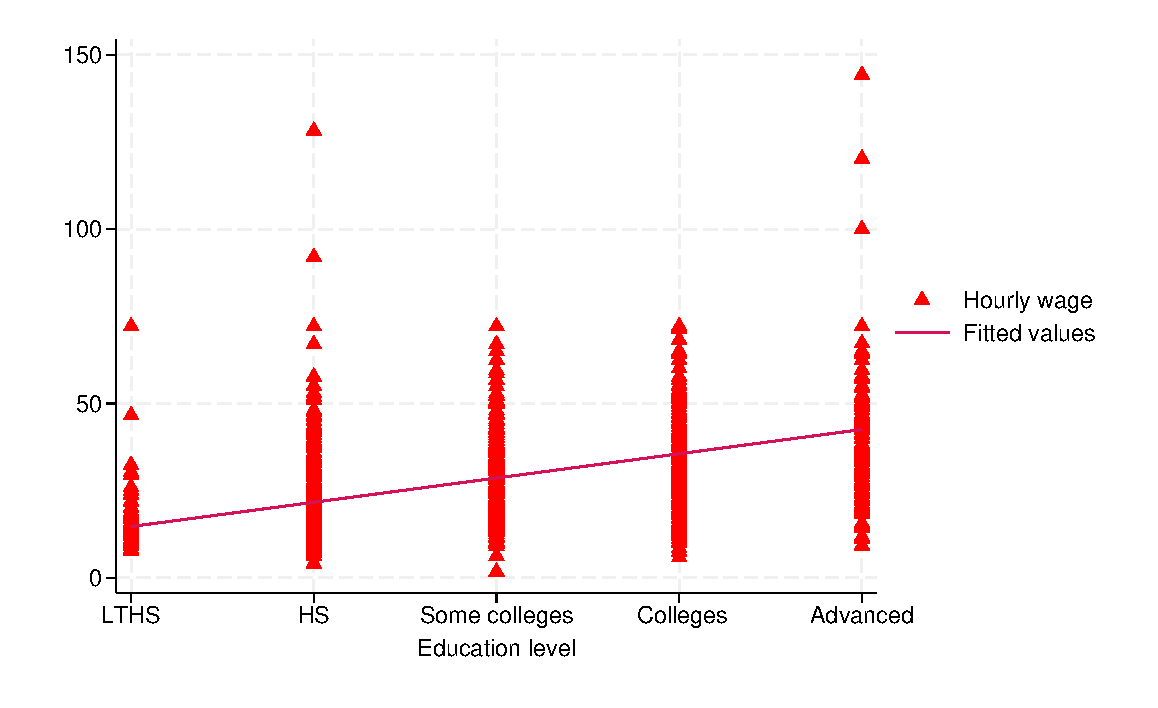
\includegraphics[scale=0.5]{Scatter plot in us 3.1.eps} %%参数表示将原图缩小或者扩大
        \caption{Scatter Plot}
        %%\label{}标签
    \end{figure}


    ii. 由CEF的分解公式知:$Y_i = E(Y_i|X_i)+\xi$。由于CEF的实际意义是在X给定的条件下,Y的均值,因此对X即教育条件进行分组求均值,得出CEF,进行OLS拟合如下图所示。
    \begin{figure}[htbp] %%图片位置,htbp分别表示在当前页,顶部,底部,浮动页
        \centering
        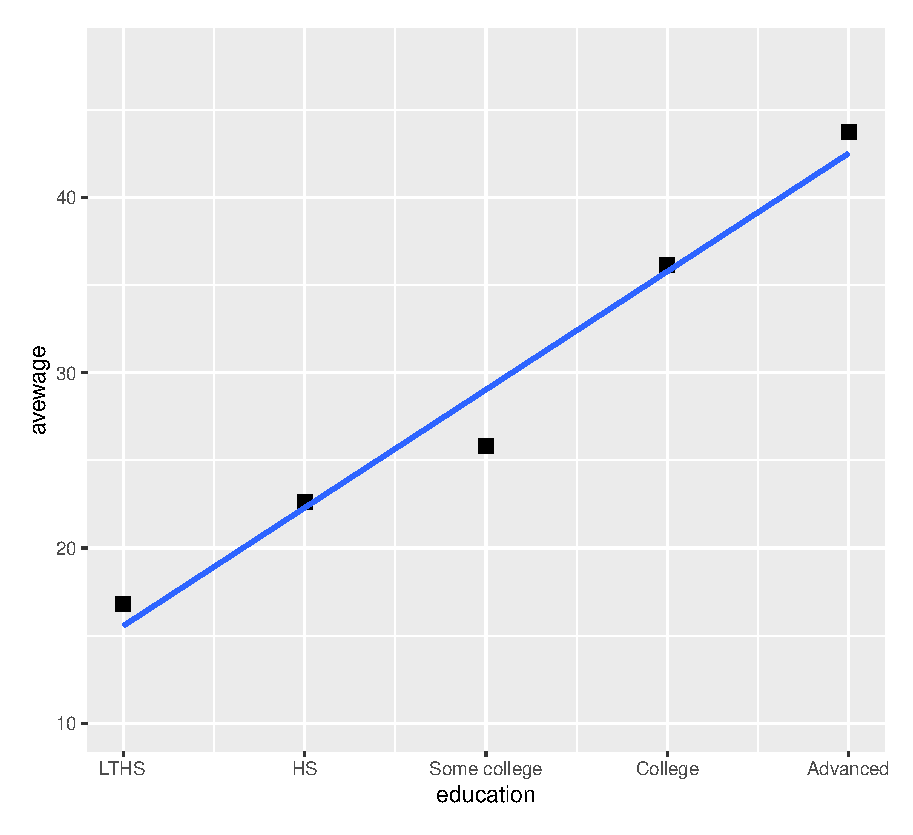
\includegraphics[scale=0.5]{R CEF.eps}
        \caption{CEF Plot}
    \end{figure}
    可以看出CEF是线性近似的,那么由CEF的回归定理,最优线性估计以及线性条件期望函数定理,总体回归方程也应该是线性近似的,且是对Y和CEF的最优线性估计量。
        \begin{equation*}
            \beta = \underset{b}{\arg \min}E{(E[Y_i|X_i] - X_i b)}
        \end{equation*}
    由上知,此种情况下CEF是线性的,则有$Y_i = X_i \beta+e_i,\beta_{OLS} -\beta =(X'X)^{-1}X'e_i$。\\
    通过变换:
    \begin{equation*}
        \beta_{OLS} -\beta =(X'X)^{-1}X'e_i=(\frac{1}{N}X'X)^{-1}\frac{1}{N}X'e_i=
        (\frac{1}{N}\sum_{i=1}^{N} X_i'X_i)^{-1}-\frac{1}{N}\sum_{i=1}^{N}X_i'e_i 
    \end{equation*}
    又因为在样本足够大时,样本均值依概率收敛于总体均值(总体矩)。则有\\
    $\frac{1}{N}\sum_{i=1}^{N} X_i'X_i\xrightarrow{P}E(X_i'X_i),\frac{1}{N}\sum_{i=1}^{N}X_i'e_i\xrightarrow{P}E(X_i'e_i)$
    又因为$E(X_i'e_i)=0$.所以有:$\beta_{OLS} -\beta\xrightarrow0$。因此OLS将会产生CEF的一致估计。

    iii. 根据条件期望的定义,有:
    \begin{tabular}[t]{l|c}
        \hline
        education & average wage \\
        \hline
        LTHS& 16.82391 \\
        HS &  22.62468\\
        Some colleges & 25.83010 \\
        College & 36.16484 \\
        Advanced & 43.75207 \\
        \hline
    \end{tabular}\\
    分别令教育水平依次从1到5进行排序,可知$D_i$表示所获教育的程度,有ols估计知\\
    容易知:
    \begin{table}[h]
        \centering
        \begin{tabular}[t]{l|c}
            \hline
            education & average wage \\
            \hline
            HS &  22.62468\\
            College & 35.24900 \\
            \hline
        \end{tabular}
    \end{table}\\
    \begin{equation*}
        D_i=
        \begin{cases*}
            1, & \text{上过大学}\\
            0, & \text{上高中未上大学}\\
        \end{cases*}
    \end{equation*}
    且$E(Y_i(0)|D_i = 1)$。表示上了大学的人如果未上大学的薪资。若无选择性偏误,那么其处理效应则是12.6,如存在选择偏误,则无法测算。
    \qedsymbol
\end{solution}

%%第四题
\item[\textbf{4.}] We wish to evaluate the effect on annual earnings of the job training provided to participants in the National Supported Work (NSW) Demonstration study. In this study, a sample of men were randomly assigned to either receive or not receive job training. Baseline earnings were measured in 1975, which is the year before the they were randomly assigned to either the treatment or control group. Earnings were also measured in 1978, which is several years after the treatment started. More details on the NSW are available in Robert Lalonde, ``Evaluating the Econometric Evaluations of Training Programs,” American Economic Review, Vol. 76, pp. 604-620.

~~The dataset for this homework is called \textbf{nsw.dta}, which can be downloaded from https://users.nber.org/$\sim$rdehejia/data/.nswdata2.html,  and includes the following variables: treatment indicator \textit{\textbf{treat}} (1 if treated, 0 if not treated), \textit{\textbf{age}} (age in years), education (years of education), \textit{\textbf{black}} (1 if black, 0 otherwise), \textit{\textbf{hispanic}} (1 if Hispanic, 0 otherwise), \textit{\textbf{married}} (1 if married, 0 otherwise), \textit{\textbf{nodegree}} (1 if no high school degree, 0 otherwise), \textit{\textbf{re75}} (earnings in 1975), and \textit{\textbf{re78}} (earnings in 1978). 

\begin{enumerate}
\item[i.] Calculate the ATE and the ATT of the policy usng a simple difference in means. How do the two values compare?
\item[ii.] Provide evidence that the randomization worked by comparing the means of the sample characteristics in the treatment and control group. Please create a clean table that includes columns with the means of each group, the difference between the two groups and the p-value of the difference. The table should be comprehensible on its own. Include a footnote for the table with a description of the dataset. A table of this form is usually the first one in an empirical study intended to recover a causal estimate. Is the table consistent with the randomization being correctly implemented?
\item[iii.]  Create a table that presents your evaluation of the effect of the NSW experiment on earnings. In the first column present the raw difference in means between the treatment and control group then sequentially add covariates. In the last column include estimates from a regression with all covariates. Do the estimates change much as you add covariates? Why or why not? What does this tell you?
\item[iv.]  Do you believe your estimates of the treatment effect are unbiased of the true treatment effect? Why or why not?
\item[v.]  Estimate and plot the density functions of the 1978 earnings for the treatment and control group.
\end{enumerate}

%%第四题解答
\begin{solution}
    i.本题假设在三年期间不存在任何其他可能影响收入的事件发生,或者说假设培训对于收入在三年间的影响是最大的。对于ATT有Rubin模型知:ATE=$E(Y_{1i}|treat_i=1)-E(Y_{0i}|treat_i=0),ATE -ATT = selection bias$。而ATT无法被直接测算出来,可以用三年前的初始收入量差距作为实验的选择偏差。\\
    数据计算得:selection bias =39.415, ATE=2949.669  ATT= 2910.254。因此ATE微大于ATT。\\

    ii. 通过数据的表格如下:\\
    \begin{table}[h]
        \centering
        \begin{threeparttable}%%[l]表示表格左对齐,[c]表示表格居中对齐,[r]表示表格右对齐
            \begin{tabular}{llll}%%l表示左对齐,c表示居中对齐,r表示右对齐,p表示百分数
                \hline
                variables & means & difference & p-value \\   
                \hline
                age0 & 24.45 & \multirow{2}{*}{0.18}  & \multirow{2}{*}{0.72} \\
                age & 24.63 &   &\\
                education0 & 10.19 & \multirow{2}{*}{0.19} & \multirow{2}{*}{0.14}\\
                education1 & 10.38 &  & \\
                black0 & 0.80 & \multirow{2}{*}{0.00} & \multirow{2}{*}{0.96} \\
                black1 & 0.80 &  &  \\
                hispanic0 & 0.11 & \multirow{2}{*}{-0.02} & \multirow{2}{*}{0.42} \\
                hispanic1 & 0.09 &  &  \\
                married0 & 0.16 & \multirow{2}{*}{0.01} & \multirow{2}{*}{0.70} \\ 
                married1 & 0.17 &  &  \\    
                nodegree0 & 0.81 & \multirow{2}{*}{-0.08} & \multirow{2}{*}{0.00} \\
                nodegree1 & 0.73 &  &  \\
                re750 & 3026.68 & \multirow{2}{*}{39.42} & \multirow{2}{*}{0.92} \\
                re751 & 3066.10 &  &   \\
                \hline
            \end{tabular} 
            \begin{tablenotes}
                \footnotesize
                    \item[1]P-value小于0.05时证明在5\%的置信区间内,差异显著
            \end{tablenotes}
        \end{threeparttable}
        \caption{\label{font-table} 随机化检验. }
    \end{table}\\
    由上表知,除了学位,其他的特征的差异都不显著,P值大于0.05。因此可以认为随机化是有效的。\\
\\
\\
\\

    iii. 由上知,75年的收入均值的差异不显著。根据stata做表得:\\
    \begin{table}[h]
        \centering
        \begin{tabular}{llll}%%l表示左对齐,c表示居中对齐,r表示右对齐,p表示百分数
            \hline
            variables & treat==0& treat==1 \\   
            \hline
            mean & 5090.048 & 5976.352 \\
            treat & \multicolumn{2}{c}{886.3037}\\
            age & \multicolumn{2}{c}{882.2074}\\
    
            education & \multicolumn{2}{c}{831.039} \\

            black & \multicolumn{2}{c}{826.4462}\\

            hispanic & \multicolumn{2}{c}{824.3952}  \\

            married & \multicolumn{2}{c}{820.4004} \\    

            re75 & \multicolumn{2}{c}{830.6734} \\   

            nodegree &\multicolumn{2}{c}{806.5113} \\
            \hline
        \end{tabular} 
        \caption{\label{font-table} 培训处理效果. }
    \end{table}\\
    由表可以看出,表中的回归系数基本变化不大,这证明基本不存在选择偏误,表明明处理效应相对稳定,不受这些协变量的影响。实验的随机化很好。
    


    iv. 由上两题知,实验的随机化水平很好,这意味着基本不存在选择偏误。那么实际的处理效应基本等于处理前后的收入的差距。由于初始的差异不显著,可以认为收入可以被很好的由是否培训的处理预测,即均值估计量差异基本无偏。
    \\
    
    v.依据数据,得出的density functions画图如下:\\
    \begin{figure}[htbp] %%图片位置,htbp分别表示在当前页,顶部,底部,浮动页
        \centering
        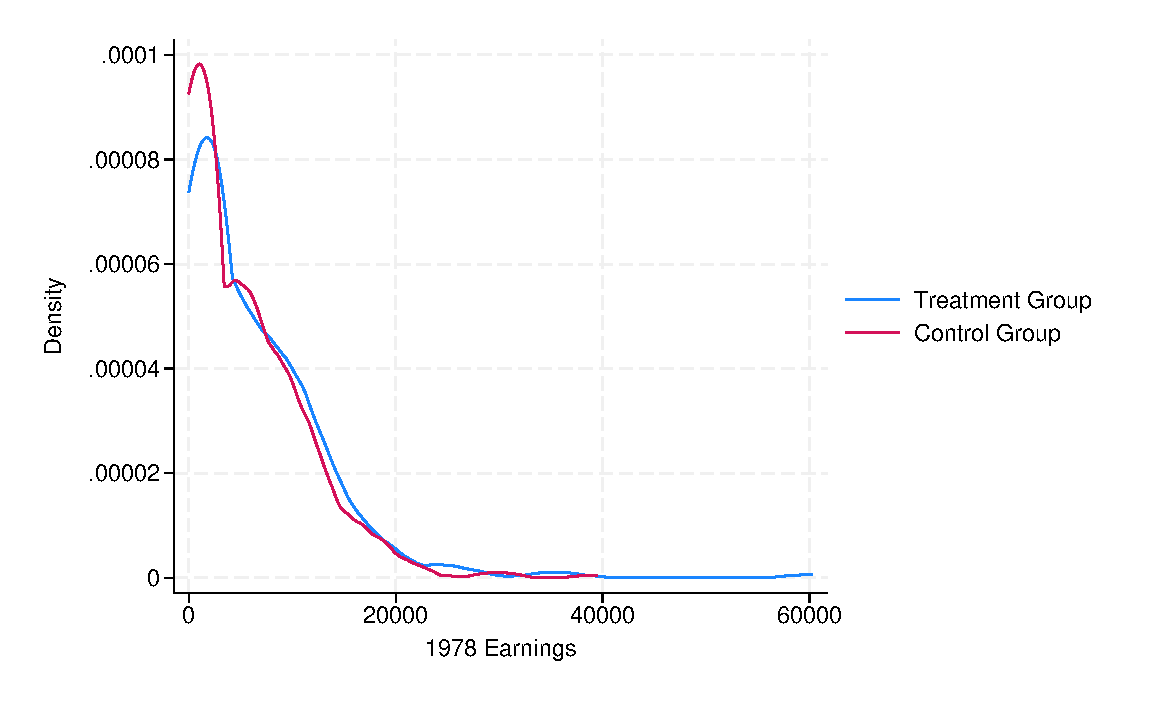
\includegraphics[scale=0.5]{density function.eps}
        \caption{Density functions}
        %%\label{}标签
    \end{figure}

    \qedsymbol
\end{solution}


%%第五题
\item[\textbf{5.}]  Duflo, Dupas, and Kremer (2011) investigate the impact of tracking (assigning students based on initial test score) on educational attainment in a randomized experiment. An extract of their data set is available on the Bruce Hansen textbook webpage in the file \textbf{DDK2011}.

~~~~In 2005, 140 primary schools in Kenya received funding to hire an extra first grade teacher to reduce class sizes. In half of the schools (selected randomly) students were assigned to classrooms based on an initial test score (``tracking''); in the remaining schools the students were randomly assigned to classrooms. For their analysis the authors restricted attention to the 121 schools which initially had a single first-grade class.
\begin{enumerate}
\item[i.] Do a regression of standardized test score (\textit{\textbf{totalscore}} normalized to have zero mean and variance 1) on tracking. Calculate standard errors using both the conventional robust formula, and clustering based on the school. Report and interpret the results.
\item[ii.]  Do a regression of standardized test score on tracking, age, gender, being assigned to the contract teacher, and student's percentile in the initial distribution. (The sample size will be smaller as some observations have missing vari- ables.) Calculate standard errors using both the conventional robust formula, and clustering based on the school. Compare the two sets of standard errors. Which standard error changes the most by clustering? Which changes the least?

\item[iii.]  How does the coefficient on tracking change by inclusion of the individual controls (in comparison to the results from i)?
\end{enumerate}



%%第五题解答
\begin{solution}
    i. 根据题意知,对于totalscore进行标准化。其次根据要求进行稳健回归,数据图如下所示:\\
    \begin{table}[h]
        \centering
        \begin{threeparttable}%%[l]表示表格左对齐,[c]表示表格居中对齐,[r]表示表格右对齐
            \begin{tabular}{llll}%%l表示左对齐,c表示居中对齐,r表示右对齐,p表示百分数
                \hline
                standardize & coefficient & Robuststd.err & P \\
                \hline
                Tracking & 0.1380913 & 0.0262102 & 0.00 \\
                cons  &  -0.0710354 & 0.0186418  & 0.00\\
                \hline
            \end{tabular} 
        \end{threeparttable}
        \caption{\label{font-table} 稳健标准误. }
    \end{table}

    \begin{table}[h]
        \centering
        \begin{threeparttable}%%[l]表示表格左对齐,[c]表示表格居中对齐,[r]表示表格右对齐
            \begin{tabular}{llll}%%l表示左对齐,c表示居中对齐,r表示右对齐,p表示百分数
                \hline
                standardize & coefficient & Robuststd.err & P \\
                \hline
                Tracking & 0.1380913 & 0.0772362 & 0.076 \\
                cons  & -0.0710354 & 0.0543934 & 0.194\\
                \hline
            \end{tabular} 
        \end{threeparttable}
        \caption{\label{font-table} 聚类稳健的标准误. }
    \end{table}
    由上表可以看出稳健的标准误以及聚类稳健的标准误情况下,系数基本没有差距,这表明分班对于测试成绩具有正向影响。同时也看出在学校层面的聚类标准误不显著,这可能是因为学校于分班存在某种相关性,导致聚类稳健的显著性下降。





    ii. 由数据回归知,
    \begin{table}[h]
        \centering
        \begin{threeparttable}%%[l]表示表格左对齐,[c]表示表格居中对齐,[r]表示表格右对齐
            \begin{tabular}{llll}%%l表示左对齐,c表示居中对齐,r表示右对齐,p表示百分数
                \hline
                standardize & coefficient & Robuststd.err & P \\
                \hline
                Tracking &  0.1725117 & 0.0761819  & 0.00 \\
                agetest  &   -0.0408029 & 0.0133116  & 0.00\\
                girl   &  0.0812035  & 0.0284988  & 0.00\\
                etpteacher   &  0.17987574 & 0.0374764    & 0.00\\
                percentile  &  0.0173172 & 0.0007203   & 0.00\\
                cons  &  -0.729054  & 0.129734  & 0.00\\
                \hline
            \end{tabular} 
        \end{threeparttable}
        \caption{\label{font-table} 聚类标准误. }
    \end{table}

    \begin{table}[h]
        \centering
        \begin{threeparttable}%%[l]表示表格左对齐,[c]表示表格居中对齐,[r]表示表格右对齐
            \begin{tabular}{llll}%%l表示左对齐,c表示居中对齐,r表示右对齐,p表示百分数
                \hline
                standardize & coefficient & Robuststd.err & P \\
                \hline
                Tracking &  0.1725117 & 0.0240222  & 0.00 \\
                agetest  &   -00408029 & 0.0084928   & 0.00\\
                girl   &  0.1798757 & 0.0240886  & 0.00\\
                etpteacher   &  0.0173172 & 0.0237054    & 0.00\\
                percentile  &  -0.0710354 & 0.0004246   & 0.00\\
                cons  &  -0.729054  & 0.0809656   & 0.00\\
                \hline
            \end{tabular} 
        \end{threeparttable}
        \caption{\label{font-table} 稳健标准误. }
    \end{table}
    观察可知,聚类标准误在各个变量方向上基本都大于稳健标准误。在进行稳健标准误之后,Tracking即是否有分班的影响。在聚类之后变化最大。



    iii.由i题和ii题comparison知,在加入个体控制变量之后。Tracking的系数有一个相对较大的上升,这表明了个体的控制变量会对于Tracking和得分之间relationship产生影响,这是由于原来作为遗漏变量的变量被重新加入回归,同时这些变量是与Tracking负相关的,这就导致加入后Tracking系数变大。
    同时也不能断定是否存在剩余的遗漏变量(未控制好随机化,可观察的变量是导致选择偏误的唯一原因)。

    \qedsymbol


\end{solution}

%%另起一page
\newpage
{\fontsize{14pt}{16pt}\selectfont \textbf{代码附录}}

{\fontsize{8pt}{12pt}\selectfont \textbf{第三题代码}}
\lstset{language=Python,basicstyle=\ttfamily\small}
    \begin{lstlisting}
        keep if female ==0&month ==3& age>30&age<40     ///&prcitshp == 1  //保留变量
        //save "C:\Users\ASUS\Desktop\Econometrics\201903 born in us.dta"  //美国国籍的人
        save "C:\Users\ASUS\Desktop\Econometrics\201903 in us.dta"


        //每次开始
        keep educ educ92 wage3 wage4 rw_ot rw //去除多余变量,看起来更加简洁    
        drop if missing(wage4, rw_ot)
        //twoway (scatter rw_ot educ, msymbol(O) mcolor(blue) msize(medium) mstyle(p9)) 
        //画图
        twoway (scatter wage4 educ, msymbol(T) mcolor(red) msize(medium) mstyle(p9)
        xlabel(1 "LTHS" 2 "HS" 3 "Some colleges" 4 " Colleges" 5 "Advanced",valuelabel))
        (lfit wage4 educ) //画图 不错


        //回归
        regress wage4 educ nonconstant
    \end{lstlisting}

{\fontsize{8pt}{12pt}\selectfont \textbf{第四题代码}}
    \begin{lstlisting}
                //ATE
        mean(re78) if treat ==1 
        mean(re75)  if treat ==0

        //ATT and selection bias
        mean(re75) if treat ==0
        mean(re75) if treat ==1 



        summarize age education black hispanic married nodegree re75 re78 if treat==0
        summarize age education black hispanic married nodegree re75 re78 if treat==1
        egen mean_age_0 = mean(age) if treat==0
        egen mean_age_1 = mean(age) if treat==1
        egen diff_age = mean_age_1 - mean_age_0
        egen mean_education_0 = mean(education) if treat==0
        egen mean_education_1 = mean(education) if treat==1
        egen diff_education = mean_education_1 - mean_education_0
        egen mean_black_0 = mean(black) if treat==0
        egen mean_black_1 = mean(black) if treat==1
        egen diff_black = mean_black_1 - mean_black_0
        egen mean_hispanic_0 = mean(hispanic) if treat==0
        egen mean_hispanic_1 = mean(hispanic) if treat==1
        egen diff_hispanic = mean_hispanic_1 - mean_hispanic_0
        egen mean_married_0 = mean(married) if treat==0
        egen mean_married_1 = mean(married) if treat==1
        egen diff_married = mean_married_1 - mean_married_0
        egen mean_nodegree_0 = mean(nodegree) if treat==0
        egen mean_nodegree_1 = mean(nodegree) if treat==1
        egen diff_nodegree = mean_nodegree_1 - mean_nodegree_0
        egen mean_re75_0 = mean(re75) if treat==0
        egen mean_re75_1 = mean(re75) if treat==1
        egen diff_re75 = mean_re75_1 -re75_0
        // 对其他变量重复上述步骤
        //t检验
        ttest age, by(treat)
        local p_age = r(p)
        ttest education, by(treat)
        local p_education = r(p)
        ttest black, by(treat)
        local p_black = r(p)
        ttest hispanic, by(treat)
        local p_hispanic = r(p)
        ttest married, by(treat)
        local p_married = r(p)
        ttest nodegree, by(treat)
        local p_nodegree = r(p)
        ttest re75, by(treat)
        local p_re75 = r(p)

        //iii
        summarize re78 if treat == 0
        summarize re78 if treat == 1
        reg re78 treat
        reg re78 treat age
        reg re78 treat age education
        reg re78 treat age education black
        reg re78 treat age education black hispanic
        reg re78 treat age education black hispanic married
        reg re78 treat age education black hispanic married re75
        reg re78 treat age education black hispanic married nodegree re75
    \end{lstlisting}

{\fontsize{8pt}{12pt}\selectfont \textbf{第五题代码}}
    \begin{lstlisting}
        //标准化
        summarize totalscore
        local mean = r(mean)
        local sd = r(sd)
        generate standardized_totalscore = (totalscore - mean) / sd
        //稳健回归
        regress standardized_totalscore tracking ,robust
        //聚类稳健的标准误
        regress standardized_totalscore tracking , vce(cluster schoolid)
        
        //删除缺失值
        drop if missing
        (standardized_totalscore, tracking ,agetest ,girl, etpteacher, percentile)
        //回归
        regress standardized_totalscore tracking agetest girl etpteacher percentile,robust
        regress standardized_totalscore tracking agetest girl etpteacher percentile 
        ,vce(cluster schoolid)
    \end{lstlisting}


\iffalse
\item \textbf{6.}
In a fit of inspiration, you devise a clever economic theory that leads to a simple regression: $y_i = \hat\alpha_1 + \hat\beta_1x_i + e_i$. You estimate the regression and are pleased to find it fits the data well: high $R_1^2$, small standard error for the slope ($s_1$). Later that night, you have a crisis of confidence: maybe you have it all backwards. Consequently, you estimate $x_i = \hat\alpha_2 + \hat\beta_2y_i+ u_i$. Your doubts are confirmed when you find this regression also fits the data well: high $R_2^2$, small standard error ($s_2$). The next morning, you set out to understand your results.
\begin{enumerate}
\item[i.] What is the relationship between $R_1^2$ and $R_2^2$?
\item[ii.]  What is the relationship between $\hat\beta_1$ and $\hat\beta_2$?
\item[iii.]  What is the relationship between $t_1 = \hat\beta_1/s_1$ and $t_2 = \hat\beta_2/s_2$?
\end{enumerate}

\item \textbf{5.} i. [\textbf{Frisch-Waugh-Lovell Theorem}] Consider the following two regression models:
\begin{align}
\bm{y}&=\bm{X_1\beta_1+X_2\beta_2+\varepsilon},\\
\bm{M_2y}& = \bm{M_2X_1\beta_1 + \varepsilon}.
\end{align}
where $\bm{M_2 = I_n-X_2(X_2^{'}X_2)^{-1}X_2^{'}}$. Show that the least squares estimator of $\bm\beta_1$ is the same in both models.

ii. Suppose we write the model as $\bm{y}=\bm{X_1\beta_1+X_2\beta_2+\varepsilon}$ and $E[\bm\varepsilon|\bm{X}] = \bm{X_1\gamma}$ for some $\bm{\gamma\neq 0}$. Is the least squares estimator of $\bm\beta_2$  biased? Prove your claim.
\fi

\end{itemize}


\end{document}